\documentclass[10pt,conference, compsocconf]{IEEEtran}

\usepackage{amsfonts}
\usepackage{amssymb,amsmath}
\usepackage{hyperref}
\usepackage{algpseudocode}
\usepackage{graphicx}
\usepackage{anyfontsize}   % for fontsize and selectfont command
\usepackage{array}         % better padding of cell content of tabulars
\usepackage[skip=2pt,font=footnotesize]{caption}

\usepackage{tikz}       % for flowcharts
\usetikzlibrary{shapes, arrows}

\newsavebox{\ieeealgbox}
\newenvironment{boxedalgorithmic}
  {\begin{lrbox}{\ieeealgbox}
   \begin{minipage}{\dimexpr\columnwidth-2\fboxsep-2\fboxrule}
   \begin{algorithmic}}
  {\end{algorithmic}
   \end{minipage}
   \end{lrbox}\noindent\fbox{\usebox{\ieeealgbox}}}

\begin{document}

\title{A shuffled complex evolution algorithm for
the multidimensional knapsack problem using core concept}

%\author{\IEEEauthorblockN{Marcos Daniel Valad\~ao Baroni}
%\IEEEauthorblockA{ Departamento de Inform\'atica\\
%Universidade Federal do Esp\'irito Santo\\
%Vit\'oria, Esp\'irito Santo, Brazil\\
%Email: mbaroni@ninfa.inf.ufes.br }
%\and
%\IEEEauthorblockN{Fl\'avio Miguel Varej\~ao}
%\IEEEauthorblockA{ Departamento de Inform\'atica\\
%Universidade Federal do Esp\'irito Santo\\
%Vit\'oria, Esp\'irito Santo, Brazil\\
%Email: fvarejao@ninfa.inf.ufes.br }
%}

\maketitle

\begin{abstract}
This work addresses the application of a population based evolutionary algorithm
called shuffled complex evolution (SCE) in the core of multidimensional knapsack
problem (MKP).
The core of the MKP is a set of items which are hard to decide if they are or
not selected in good solutions.
This concept is used to reduce the original size of MKP instances.
%The SCE regards a natural evolution happening simultaneously in independent communities.
The performance of the SCE applied to the reduced MKP is verified through computational experiments
using well-known instances from literature.
The approach proved to be very effective in finding near optimal solutions
demanding a very small amount of processing time.
\end{abstract}
\IEEEpeerreviewmaketitle

\section{Introduction}
\label{sec:intro}

The multidimensional knapsack problem (MKP) is a strongly NP-hard combinatorial
optimization problem which can be viewed as a resource allocation problem and
defined as follows:

\begin{align*}
  \text{maximize} & \sum_{j=1}^n p_j x_j \\
  \text{subject to} & \sum_{j=1}^n w_{ij} x_j \leqslant c_i \quad i \in \{1, \ldots, m\}\\
   & x_j \in \{0, 1\}, \quad j \in \{1, \ldots, n\}.
\end{align*}

% Define the MKP
The problem can be interpreted as a set of $n$ items with profits $p_j$
and a set of $m$ resources with capacities $c_i$.
Each item $j$ consumes an amount $w_{ij}$ from each resource $i$, if selected.
The objective is to select a subset of items with maximum total profit,
not exceeding the defined resource capacities.
The decision variable $x_j$ indicates if $j$-th item is selected.

The multidimensional knapsack problem can be applied on budget planning 
scenarios, subset project selections, cutting stock problems, task scheduling,
allocation of processors and databases in distributed computer programs.
The problem is a generalization of the well-known knapsack problem (KP) in which
$m = 1$.

The MKP is a NP-hard problem significantly harder to solve in practice than the KP.
Despite the existence of a fully polynomial approximation scheme (FPAS) for the KP,
finding a FPAS for the MKP is NP-hard for $m \geqslant 2$~\cite{magazine1984note}.
Due its simple definition but challenging difficulty the MKP is often used to
to verify the efficiency of novel metaheuristics.

Its well known that the hardness of a NP-hard problem grows exponentially over
its size.
Thereupon, a suitable approach for tackling those problems is to reduce their size
through some variable fixing procedure.
Despite not guaranteeing optimality of the solution, an efficient variable
fixing procedure may provide near optimal solutions through a small computational effort.

%A metaheuristic is a set of concepts that can be used to define heuristic methods
%that can be applied to a wide set of different problems.
%In other words, a metaheuristic can be seen as a general algorithmic framework which can be applied to
%different optimization problems with relatively few modifications to make them adapted to a specific problem.”

The SCE is a metaheuristic, proposed by Duan in \cite{duan1992effective},
which combines the ideas of a controlled random search with the concepts
of competitive evolution and shuffling.
The SCE algorithm has been successfully used to solve several problems
like flow shop scheduling~\cite{zhao2014shuffled} and project management~\cite{elbeltagi2007modified}.

In this paper we address the development of a hybrid heuristic for the MKP.
The size of the problem instance is first reduced through a variable fixing
procedure that uses a known concept among knapsack problems called \emph{core}.
The reduced problem is then efficiently solved by a SCE algorithm.

The reminder of the paper is organized as follows:
Section~\ref{sec:core} defines the core concept for the MKP and its application
for the problem reduction.
Section~\ref{sec:sce} presents the shuffled complex evolution algorithm
and proposes its application on the MKP.
Section~\ref{sec:exp} comprises several computational experiments over well-known
instances from literature.
In section~\ref{sec:conc} we make our concluding remarks about the developed
methods and the experimental results.



\section{The core concept for MKP}
\label{sec:core}
The core concept was first presented for the one-dimensional 0-1 knapsack problem (KP),
leading to very successful KP algorithms.
The main idea is to reduce the original problem by only considering a set of
items for which it is hard to decide if they will occur or not in an optimal solution.
This set of items is named core.
The variables for all items outside the core are fixed to certain values.

The KP considers items $j = 1, \ldots, n$, associated profits $p_j$ and
associated weights $w_j$.
A subset of these items has to be selected and packed into a knapsack having capacity $c$.
The total profit of the items in the knapsack has to be maximized, while the
total weight is not allowed to exceed $c$.

If the items are sorted according to descreasing efficiency values
\begin{displaymath}
  e_j = \frac{p_j}{w_j},
\end{displaymath}
it is well known that the solution of the LP-relaxation consists in general of
three consecutive parts: The fisrt part contains variables set to $1$, the second
pare consists of at most on split item $s$, whose corresponding LP-values is
factional, and finally the remaining variables, which are always set to zero,
form the third part.
For most instance of KP (except those with a very special structure) the integer
optimial solution closely corresponds to this partitioning in the sense that it
contains most of the highly efficient items of the first part, some items with
medium efficiencies near the split item, and almost no items with low efficiencies
from the third part.
Items of medium efficiency constitute the so called core.

Balas and Zemel~\cite{balas1980algorithm} gave the following precise definition
of the core of a KP, based on the knowledge of an optimal integer solution $x^*$.
Assume that the items are sorted according to descreasing efficiencies and let
\begin{displaymath}
  a := \min\{ j | x_k^* = 0 |\}, \quad b := \max\{ j | x_j^* = 1 \}.
\end{displaymath}
The core is given by the items in the interval $C = \{a, \ldots, b\}$.
It is obvious that the split item is always part of the core.

The KP Core problem (KPC) is defined as
\begin{align*}
  \text{maximize} & \sum_{j \in C} p_j x_j  + \tilde{p}\\
  \text{subject to} & \sum_{j \in C} w_{j} x_j \leqslant c - \tilde{w}\\
  & x_j \in \{0, 1\}, \quad j \in C.
\end{align*}
with $\tilde{p} = \sum^{a-1}_{j=1} p_j$  and $\tilde{w} = \sum^{a-1}_{j=1} w_j$.
The solution of KPC would suffice to compute teh optimal solution of KP, which
however, has to be already partially known to determine $C$.
Nevertheless an approximate core of fixed size $c = \{s-\lambda, \ldots, s+\lambda\}$,
given a $\lambda$, can be considered for a heuristic reduction of MKP problem.

\subsection{The Core Concept for MKP}

The previous definition of the core for KP can be expanded to MKP without major difficulties,
once an efficiency measure $e$ is defined for the MKP,
as presented by Puchinger, Raidl and Pferschy~\cite{puchinger2006core}.
Although an efficiency measure for MKP is not obvious due the
multidimensional weight of the items.

In \cite{puchinger2006core} various proposals for efficiency measure was
investigated and...
\begin{displaymath}
  e = \frac{p_j}{\sum_{i=1}^m r_iw_{ij}}
\end{displaymath}
where $r_i$ are set to the values of an optimal solution to the dual problem of
the MKP's LP-relaxation, as suggested in \cite{Chu-Beasley-1998}.

Let $x^*$ be an optimal solution and assume that the items are sorted according
to decreasing efficiency $e$, then let
\begin{displaymath}
  a_e = \min \{ j | x_j^* = 0 \}, \quad b_e = \max \{ j | x_j^* = 1 \}.
\end{displaymath}
The core is given by the items in the interval $C_e = \{ a_e, \ldots, b_e \}$,
and the multidimensional knapsack core problem (MKPC) defined as
\begin{align*}
  \text{maximize} & \sum_{j \in C} p_j x_j  + \tilde{p}\\
  \text{subject to} & \sum_{j \in C} w_{ij} x_j \leqslant c_i - \tilde{w}_i, \quad i = 1, \ldots, m\\
  & x_j \in \{0, 1\}, \quad j \in C.
\end{align*}
with $\tilde{p} = \sum^{a-1}_{j=1} p_j$  and $\tilde{w}_i = \sum^{a-1}_{j=1} w_{ij}, i = 1, \ldots, m$.

In contrast to KP, the solution of the LP-relaxation of MKP in general does not
consists of a single fractional split item. But up to $m$ fractional values give
rise to a whole split interval $S_e = \{ s_e, \ldots, t_e \}$, where
$s_e$ and $t_e$ are the first and the last index of variables with fractional
values after sorting by efficiency $e$.



\cite{puchinger2006core}

% - Eficieny measure...
% - the core problem (KPC)
% - core concept for MKP
%  - Efficiency measure... (sketch...) the dual efficieny measure
%  - the Multidimentional kanspack core problem (MKPC)



\section{The shuffled complex evolution for the MKP}
\label{sec:sce}
The shuffled complex evolution is a population
based evolutionary optimization algorithm that regards a natural 
evolution happening simultaneously in independent communities.
The algorithm works with a population partitioned in $N$ complexes, each one
having $M$ individuals.
In the next Subsection the SCE is explained in more details.
In the later Subsection the application of SCE to the multidimensional knapsack
problem is considered.
% In the SCE the population is partitioned into communities (complexes), each of which
% will evolve independently through a number of evolving steps.
% In each evolving step a subset of the complex (subcomplex) is selected as potencial group of
% parents.

%To avoid been trapped in local optimum a new offspring can be occasionally taken
%from a random location of the feasible space and introduced to the complex.

\subsection{The shuffled complex evolution}
In the SCE a population of $N*M$ individuals is randomly taken from the
feasible solution space.
After this initialization the population is sorted by descending order according
to their fitness and the best global solution is identified.
The entire population is then partitioned (shuffled) into $N$ complexes,
each containing $M$ individuals.
In this shuffling process the first individual goes to the first complex, the second
individual goes to the second complex, individual $N$ goes to $N$-th complex,
individual $M+1$ goes back to the first complex, etc.

The next step after shuffling the complexes is to evolve each complex through
a given fixed amount of $K'$ steps.
The individuals in each complex is sorted by descending order of fitness quality.
In each step a subcomplex of $P$ individuals is selected from the
complex using a triangular probability distribution, where the $i$-th individual
has a probability $p_i = \frac{2(n+1-i)}{n(n+1)}$ of being selected.
The use of triangular distribution is intended to prioritize individuals with
better fitness, supporting the algorithm convergence rate.

After the selection of the subcomplex, its worst individual is identified to
be replaced by a new generated solution.
This new solution is generated by the crossing of the worst individual and an
other individual with better fitness.
At first the best individual of the subcomplex is considered for the crossing.
If the new solution is not better than the worst one, the best individual
of the complex is considered for a crossing.
If the latter crossing did not result in any improvement, the best individual
of whole population is considered.
Finally, if all the crossing steps couldn't generate a better individual,
the worst individual of the subcomplex is replaced by a new random solution taken
from the feasible solution space.
This last step is important to prevent the algorithm becoming trapped in local minima.
Fig.~\ref{fig:flow2} presents the evolving procedure described above in a flowchart diagram.

After evolving all the $N$ complexes the whole population is again
sorted by descending order of fitness quality and the process continues until
a stop condition is satisfied.
Fig.~\ref{fig:flow1} shows the SCE algorithm in a flowchart diagram.

\begin{figure}[htp]
  \subfigure[The SCE algorithm overview.]{
    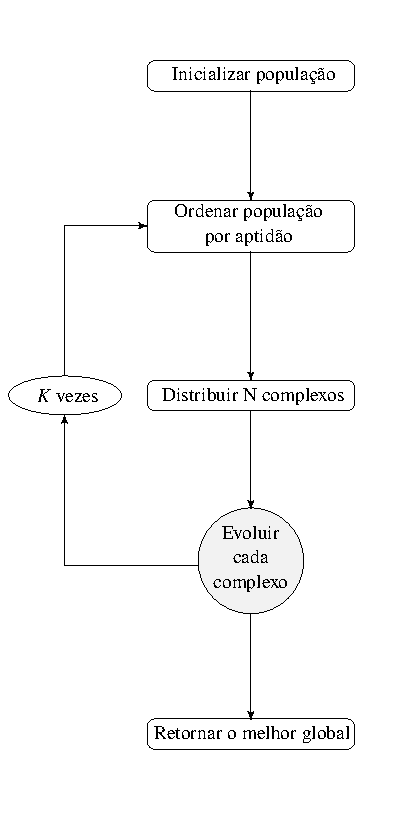
\includegraphics[width=0.47\linewidth]{imgs/flow1}
    \label{fig:flow1}
  }
  ~
  \subfigure[Evolving stage for a single complex.]{
    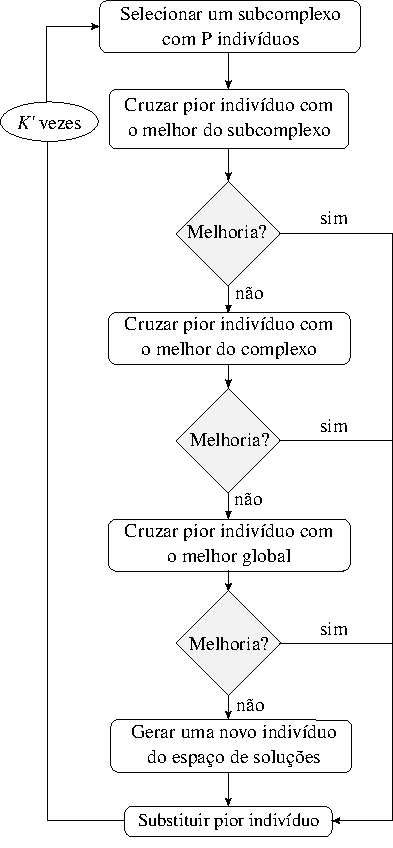
\includegraphics[width=0.47\linewidth]{imgs/flow2}
    \label{fig:flow2}
  }
  \caption{Flowchart representing the shuffled complex evolution algorithm.}
  \label{fig:sce}
\end{figure}


\subsection{The shuffled complex evolution for the MKP}

As it can be noted in its description the SCE is easly applied to any
optimization problem.
The only steps needed to be specified is (a) the creation of a new random
solution and (b) the crossing procedure of two solutions.
These two procedures are respectively presented by Algorithm.~\ref{alg:new} and
Algorithm~\ref{alg:cross}.

\begin{algorithm}
\begin{algorithmic}[1]
  \Procedure{New random solution}{}
    \State $v \leftarrow $ shuffle($1, 2, \ldots, n$)
	\State $s \leftarrow \emptyset$ \Comment{empty solution}
    \For{$ i \leftarrow 1:n$ }
	  \State $s \leftarrow s \cup \{v_i\}$ \Comment{adding item}
	  \If{ $s$ is not feasible} \Comment{checking feasibility}
	    \State $s \leftarrow s - \{v_i\}$
      \EndIf
	\EndFor
  \State return $s$
  \EndProcedure
\end{algorithmic}
\caption{Generation of a new random solution for the MKP.}
\label{alg:new}
\end{algorithm}

To construct a new random solution (Algorithm~\ref{alg:new}) the items are
at first shuffled in random order and stored in a list (line 2).
A new empty solution is then defined (line 3).
The algorithm iteratively tries to fill the solution's knapsack with 
the an item taken from the list (lines 4-9).
The feasibility of the solution is then checked: if the item insertion let
the solution unfeasible (line 6) its removed from knapsack (line 7).
After trying to place all available items the new solution is returned.

\begin{algorithm}
\begin{algorithmic}[1]
  \Procedure{Crossing}{$x^w:$ worst individual, $x^b:$ better individual, $c$}
    \State $v \leftarrow $ shuffle($1, 2, \ldots, n$)
    \For{$ i \leftarrow 1:c$ }
	  \State $j \leftarrow v_i$
	  \State $x^w_j \leftarrow x^b_j$ \Comment{gene carriage}
	\EndFor
	\If{$s^w$ is not feasible}
	  \State repair $s^w$
	\EndIf
	\State update $s^w$ fitness
  \State return $s^w$
  \EndProcedure
\end{algorithmic}
\caption{Crossing procedure used on SCE algorithm.}
\label{alg:cross}
\end{algorithm}

The crossing procedure (Algorithm~\ref{alg:cross}) takes as input the worst
solution taken from the subcomplex $x^w = (x^w_1, x^w_2, \ldots, x^w_n$),
the selected better solution $x_b = (x^b_1, x^b_2, \ldots, x^b_n$)
and the number $c$ of genes that will be carried from the better solution.
The $c$ parameter will control how similar the worst individual will be from the
given better individual.
At first the items are shuffled in random order and stored in a list (line 2).
Then $c$ randomly chosen genes are carried from the better individual to the worst
individual (line 5).
At the end of steps the feasibility of the solution is checked (line 7) and
the solution is repaired if needed.
The repair stage is a greedy procedure that iteratively removes the item that less
decreases the objective function.
Finally the fitness of the generated solution is updated (line 10) and
returned (line 11).

%\begin{algorithmic}
%  \Procedure{The SCE for the MKP}{$\vec{p}, W, \vec{b}$}
%    \State Inicialize population
%    \For{$ i \leftarrow 1:K$ }
%	  \State Sort population by fitness
%	  \State $s_{gb} \leftarrow$ Global best individual
%	  \State Shuffle complexes
%      \For{ each complex }
%	    \State $s_{cb} \leftarrow$ Complex best individual
%        \For{$ k \leftarrow 1:K'$ }
%		  \State Select a subcomplex of $P$ individuals
%          \State $s_w \leftarrow$ worst individual of subcomplex
%          \State $s_b \leftarrow$ best individual of subcomplex
%		  \State $s_{new} \leftarrow s_w \otimes s_b$
%		  \If{ $fitness(s_{new}) > s_w$}
%		    \State $s_w \leftarrow s_{new}$
%		  \Else
%		    \State $s_{new} \leftarrow s_w \otimes s_{cb}$
%		    \If{ $fitness(s_{new}) > s_w$}
%		      \State $s_w \leftarrow s_{new}$
%			\Else
%		      \State $s_{new} \leftarrow s_w \otimes s_{gb}$
%		      \If{ $fitness(s_{new}) > s_w$}
%		        \State $s_w \leftarrow s_{new}$
%		      \Else
%			    \State $s_w \leftarrow$ new random solution
%			  \EndIf
%		    \EndIf
%		  \EndIf
%        \EndFor
%      \EndFor
%    \EndFor
%	\State $s_gb \leftarrow$ Global best individual
%	\State Return $s_gb$
%  \EndProcedure
%\end{algorithmic}

%\begin{algorithmic}
%  \Procedure{New random MKP solution}{$\vec{p}, W, \vec{b}$}
%    \State $\vec{v} \leftarrow $ shuffle$(1, 2, \ldots, n)$
%	\State $s \leftarrow \emptyset $
%    \For{$ i \leftarrow 1:niter$ }
%	  \If{$ s \cup \{v[i]\} is feasible$}
%	    \State $s \leftarrow s \cup \{v[i]\}$
%	  \EndIf
%    \EndFor
%  \EndProcedure
%\end{algorithmic}


\section{Computational experiments}
\label{sec:exp}
To verify the efficiency of the proposed hybrid metaheuristic, several computational
experiments was executed considering the original SCE for the MKP proposed in
\cite{baroni2015shuffled} and the hybrid SCE, proposed in this work.
For brevity the hybrid SCE proposed in this work will be referred to as \scecore.

For the experiments, two sets of MKP instances was used:
a first set composed by 270 instances provided by Chu and Beasley (\cite{Chu-Beasley-1998})
and a second set composed by 11 instances provided by Glover and Kochenberger in
\cite{glover1996critical}.
These instances are all available at \cite{ORLibrary}.

The best known solution for all instances were taken from the literature and
were found by different algorithms which we had no access to the implementation.
In mosts cases those are exact algorithms which took
minutes or hours of execution time.

The set of MKP instances provided by Chu and Beasley was generated using a
procedure suggested by Freville and Plateau~\cite{freville1994efficient}, which
attempts to generate instances hard to solve.
The number of constraints $m$ varies among $5$, $10$ and $30$, and the number
of variables $n$ varies among $100$, $250$ and $500$.

The $w_{ij}$ were integer numbers drawn from the discrete uniform distribution
$U(0, 1000)$.
The capacity coefficient $c_i$ were set using
$b_i = \alpha\sum_{j=1}^{n} w_{ij}$ where $\alpha$ is a tightness ratio and
varies among $0.25$, $0.5$ and $0.75$.
For each combination of $(m,n,\alpha)$ parameters, $10$ random problems was generated,
totaling $270$ problems.
The profit $p_j$ of the items were correlated to $w_{ij}$ and generated as follows:
\begin{displaymath}
  p_j = \sum_{i=1}^m \frac{w_{ij}}{m} + 500q_j \qquad j = 1, \ldots, n
\end{displaymath}

%\subsection{The set of random instances}

%The second set of instances is composed by problems generated using a similar
%setup.
%The only differences is that the profit $p_j$ is also drawn from a discrete uniform
%distribution $U(0, 1000)$.
%For each combination of $(m, n, \alpha)$ parameter, $600$ random problems was
%generated, totaling $16200$ problems.

\subsection{Experimental results}

All the experiments were run on a Intel$^R$ Core i5-3570 CPU @3.40GHz computer
with 4GB of RAM.
The original SCE and \scecore was both implemented in C programming language.
%For the set of random instance all best known solution was found by the solver
%SCIP 3.0.1 running for at least 10 minutes.

For the variable fixing procedure used on \scecore, the range size of the approximate core was
$|C| = m+\frac{n}{10}$ for all instances.
In all instances the parameters used for SCE and \scecore were the same recommended
in \cite{baroni2015shuffled} which was found after a batch test using Chu and Beasley instances:
\begin{itemize}
  \item $N = 20$: number of complexes;
  \item $M = 20$: number of individuals in each complex;
  \item $P = 5$: number of individuals in each subcomplex;
  \item $K = 300$: number of algorithm iterations;
  \item $K' = 20$: number of iterations used in the complex evolving process;
  \item $c = n/5$: number of genes carried from parent in crossing process.
\end{itemize}

Table~\ref{tab:chu} shows the performance of the SCE and \scecore on the Chu-Beasley set of instances.
Each instance in the set was executed 10 times for each algorithm.
Columns \textit{n}, \textit{m} and \textit{$\alpha$} shows the parameters used
on each instance generation.
The \textit{time} column shows the average execution time of the algorithms (lower is better).
The \textit{quality} column shows the average ratio of the solution found and
the best known solution from literature (\cite{vimont2008reduced, della2012improved}) of each instance (higher is better).

It can be observed that the \scecore had faster convergence speed, achieving higher
quality solutions in all cases, achieving at least $99.02\%$ of best known, in less than $2$ seconds
for every instance.

It can be also noticed that \scecore executed in much less processing time than original
SCE.
This is due the variable fixing procedure which reduced the problem size,
resulting in less genes operations during the evolving procedures.
The variable fixing procedure also brought robustness for the method, as the quality
of the solution found increased in case of larger instances while on original
SCE the quality decreased considerably.

\begin{table}
{
\renewcommand{\arraystretch}{1.3}%
\fontsize{8.5pt}{1em}\selectfont 
\begin{center}
  \begin{tabular}{|r|r|r|rr|rr|} \cline{4-7}
  \multicolumn{3}{c|}{} &  \multicolumn{2}{c|}{\bf time (s)} & \multicolumn{2}{c|}{\bf quality (\%)} \\ \hline
\textbf{n}   & \textbf{m}  & \textbf{$\alpha$} &
  \textbf{SCE} & \textbf{\scecore} & {\bf SCE} & {\bf \scecore}  \\ \hline
100 &  5 & 0.25 & 0.79 & 0.15 & 96.5 & 99.73 \\
    &    & 0.50 & 0.81 & 0.15 & 97.4 & 99.86 \\
    &    & 0.75 & 0.83 & 0.13 & 98.9 & 99.91 \\ \cline{2-7}
    & 10 & 0.25 & 0.75 & 0.22 & 95.7 & 99.53 \\
    &    & 0.50 & 0.93 & 0.22 & 96.7 & 99.76 \\
    &    & 0.75 & 0.89 & 0.22 & 98.5 & 99.96 \\ \cline{2-7}
    & 30 & 0.25 & 1.01 & 1.00 & 95.4 & 99.02 \\
    &    & 0.50 & 1.07 & 0.79 & 96.4 & 99.21 \\
    &    & 0.75 & 0.99 & 0.77 & 98.2 & 99.52 \\ \cline{2-7}
    & \multicolumn{2}{r|}{\textbf{average}}  & 0.90 & {\bf 0.41} & 97.5 & {\bf 99.50} \\ \hline
250 &  5 & 0.25 & 1.72 & 0.54 & 93.2 & 99.87 \\
    &    & 0.50 & 1.75 & 0.55 & 94.9 & 99.94 \\
    &    & 0.75 & 1.78 & 0.51 & 97.6 & 99.95 \\ \cline{2-7}
    & 10 & 0.25 & 1.84 & 0.67 & 93.1 & 99.57 \\
    &    & 0.50 & 1.84 & 0.62 & 94.6 & 99.80 \\
    &    & 0.75 & 1.81 & 0.64 & 97.2 & 99.88 \\ \cline{2-7}
    & 30 & 0.25 & 2.21 & 1.16 & 93.2 & 99.46 \\
    &    & 0.50 & 2.21 & 0.96 & 94.2 & 99.36 \\
    &    & 0.75 & 2.31 & 1.03 & 96.6 & 99.59 \\ \cline{2-7}
    & \multicolumn{2}{r|}{\textbf{average}} & 1.94 & {\bf 0.74} & 95.0 & {\bf 99.60} \\ \hline
500 &  5 & 0.25 & 3.16 & 0.85 & 91.4 & 99.77 \\
    &    & 0.50 & 3.18 & 0.86 & 93.4 & 99.87 \\
    &    & 0.75 & 3.34 & 0.84 & 96.4 & 99.92 \\ \cline{2-7}
    & 10 & 0.25 & 3.39 & 0.99 & 91.7 & 99.49 \\
    &    & 0.50 & 3.37 & 0.97 & 93.1 & 99.78 \\
    &    & 0.75 & 3.44 & 0.95 & 96.2 & 99.83 \\ \cline{2-7}
    & 30 & 0.25 & 3.83 & 1.53 & 91.4 & 99.75 \\
    &    & 0.50 & 3.90 & 1.48 & 92.6 & 99.42 \\
    &    & 0.75 & 3.99 & 1.42 & 96.0 & 99.68 \\ \cline{2-7}
    & \multicolumn{2}{r|}{\textbf{average}} & 3.51 & {\bf 1.10} & 93.58 & {\bf 99.61} \\ \hline
\end{tabular}

\end{center}
}
 \caption{SCE and \scecore  performance on Chu-Beasley problems.}
 \label{tab:chu}
\end{table}

Table~\ref{tab:gk} shows the performance of SCE and \scecore on the Glover-Kochenberger set of instances.
Each instance in the set was executed 10 times for each algorithm.
Columns \textit{n} and \textit{m} indicate the size of each instance.
The \textit{time} column shows the average execution (lower is better).
The \textit{quality} column shows the average ratio of the solution found and
the best known solution of each instance.
It can be noticed that SCEcr achieved high quality solutions, at least $99.10\%$
of best known solution, spending very small amount of processing time, compared
to the time taken to find the best known solutions.

\begin{table}
{
\renewcommand{\arraystretch}{1.7}%
\fontsize{8.5pt}{1em}\selectfont 
\begin{center}
\begin{tabular}{|r|r|r|r|r|r|r|} \cline{4-7}
		\multicolumn{3}{c|}{} & \multicolumn{2}{c|}{\bf time (s)} & \multicolumn{2}{c|}{\bf quality (\%)} \\ \hline
		\textbf{\#} & \textbf{n}   & \textbf{m}  & {\bf SCE } & {\bf SCEcr } & {\bf SCE} & {\bf SCEcr} \\ \hline
01 & 100 & 15 & 1.48   & 0.31 & 97.67 &  99.68 \\ \hline
02 & 100 & 25 & 1.60   & 0.47 & 97.93 &  99.51 \\ \hline
03 & 150 & 25 & 2.48   & 0.79 & 97.25 &  99.60 \\ \hline
04 & 150 & 50 & 3.44   & 1.61 & 97.38 &  99.10 \\ \hline
05 & 200 & 25 & 3.30   & 0.83 & 96.89 &  99.73 \\ \hline
06 & 200 & 50 & 4.26   & 1.67 & 97.69 &  99.30 \\ \hline
07 & 500 & 25 & 6.74   & 1.27 & 97.12 &  99.72 \\ \hline
08 & 500 & 50 & 11.23  & 2.06 & 97.29 &  99.62 \\ \hline
09 &1500 & 25 & 22.28  & 1.83 & 96.90 &  99.32 \\ \hline
10 &1500 & 50 & 31.60  & 5.25 & 97.49 &  99.76 \\ \hline
11 &2500 &100 &107.76  &11.94 & 97.94 & 99.77 \\ \hline
    \multicolumn{3}{|r|}{\textbf{average }} & {17.83} & \multicolumn{1}{r|}{\bf 2.55 } & {97.41} & {\bf 99.46}  \\ \hline
\end{tabular}
\end{center}
}
 \caption{\scecore performance on Glover-Kochenberger problems.}
 \label{tab:gk}
\end{table}

%\begin{table}
%{
%\renewcommand{\arraystretch}{1.5}%
%\fontsize{8.5pt}{1em}\selectfont 
%\begin{center}
%\begin{tabular}[c]{|r|r|r|rrr|} \hline
%\textbf{n}   & \textbf{m}  & \textbf{$\alpha$}    &\textbf{SCIP time (s)}& \textbf{SCE time (s)} & \textbf{gap (\%)} \\ \hline
%100 &  5 & 0.25 & $  0.93$ & $  0.41$  & $98.3$ \\
%    &    & 0.50 & $  0.28$ & $  0.39$  & $99.3$ \\
%    &    & 0.75 & $  0.09$ & $  0.37$  & $99.8$ \\ \cline{2-6}
%    & 10 & 0.25 & $  3.15$ & $  0.41$  & $98.2$ \\
%    &    & 0.50 & $  0.71$ & $  0.40$  & $99.3$ \\
%    &    & 0.75 & $  0.16$ & $  0.37$  & $99.8$ \\ \cline{2-6}
%    & 30 & 0.25 & $  7.26$ & $  0.42$  & $98.3$ \\
%    &    & 0.50 & $  1.47$ & $  0.42$  & $99.3$ \\
%    &    & 0.75 & $  0.25$ & $  0.38$  & $99.8$ \\ \cline{2-6}
%    & \multicolumn{4}{r}{\textbf{average gap}}  & $\bf 99.1$  \\ \hline \hline
%\textbf{n}   & \textbf{m}  & \textbf{$\alpha$}    &\textbf{SCIP time (s)}& \textbf{SCE time (s)} & \textbf{gap (\%)} \\ \hline
%250 &  5 & 0.25 & $ 58.20$ & $  1.10$  & $97.2$ \\
%    &    & 0.50 & $  8.51$ & $  1.04$  & $98.9$ \\
%    &    & 0.75 & $  0.51$ & $  0.90$  & $99.7$ \\ \cline{2-6}
%    & 10 & 0.25 & $227.94$ & $  1.11$  & $97.6$ \\
%    &    & 0.50 & $ 43.69$ & $  1.02$  & $99.0$ \\
%    &    & 0.75 & $  1.59$ & $  0.90$  & $99.8$ \\ \cline{2-6}
%    & 30 & 0.25 & $270.48$ & $  1.20$  & $97.7$ \\
%    &    & 0.50 & $ 88.73$ & $  1.09$  & $99.0$ \\
%    &    & 0.75 & $  2.90$ & $  0.94$  & $99.8$ \\ \cline{2-6}
%    & \multicolumn{4}{r}{\textbf{average gap}}  & $\bf 98.7$  \\ \hline \hline
%\textbf{n}   & \textbf{m}  & \textbf{$\alpha$}    &\textbf{SCIP time (s)}& \textbf{SCE time (s)} & \textbf{gap (\%)} \\ \hline
%500 &  5 & 0.25 & $278.85$ & $  2.23$  & $96.1$ \\
%    &    & 0.50 & $177.32$ & $  2.14$  & $98.4$ \\
%    &    & 0.75 & $  8.47$ & $  1.87$  & $99.6$ \\ \cline{2-6}
%    & 10 & 0.25 & $284.11$ & $  2.30$  & $96.7$ \\
%    &    & 0.50 & $275.68$ & $  2.16$  & $98.6$ \\
%    &    & 0.75 & $ 33.67$ & $  1.90$  & $99.7$ \\ \cline{2-6}
%    & 30 & 0.25 & $283.78$ & $  2.50$  & $96.9$ \\
%    &    & 0.50 & $283.54$ & $  2.32$  & $98.7$ \\
%    &    & 0.75 & $ 71.66$ & $  1.96$  & $99.7$ \\ \cline{2-6}
%    & \multicolumn{4}{r}{\textbf{average gap}}  & $\bf 98.3$  \\ \hline
%\end{tabular}
%\end{center}
%}
% \caption{SCE performance on the random generated problems.}
% \label{tab:rand}
%\end{table}

%\begin{figure}
%  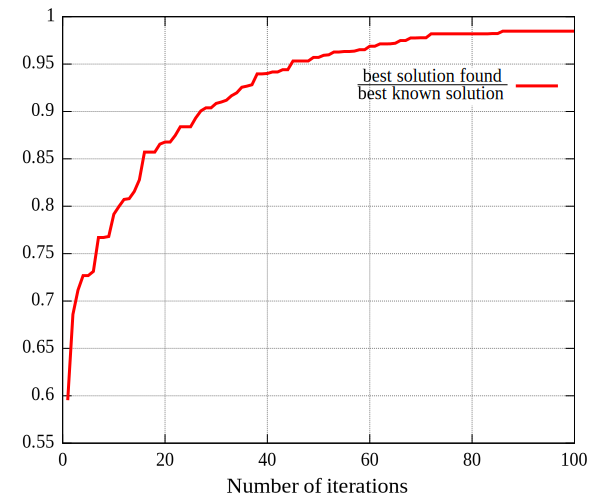
\includegraphics[scale=0.5]{imgs/iter}
%  \caption{Convergence process of SCE for MKP
%    for a problem with $n=500$, $m=30$ and $t=0.50$.}
%  \label{fig:iter}
%\end{figure}

%The fast convergence speed of SCE for MKP can be noticed in Fig.~\ref{fig:iter}.
%The figure shows for each iterations step, the quality of best solution found
%for the first $100$ iterations.
%The problem instance used was taken from the second set of problem (random instances).
%The best known solution was found with $600$s of execution on SCIP solver and
%the execution of the SCE algorithm expended $1.1$ seconds.



\section{Conclusions and future remarks}
\label{sec:conc}

In this paper we addressed the development of a hybrid heuristic for the MKP
implementing a population based algorithm called shuffled complex evolution
for solving the multidimensional knapsack problem assisted by an efficient
variable fixing procedure.
Its performance was verified through several computational experiments.

The SCE algorithm, which combines the ideas of a controlled random search with
the concepts of competitive evolution, proved to be able to achieve fast
convergence ratio, finding good quality near optimal solutions, demanding small
amount of computational time.

The application of the core concept, through a variable fixing procedure for MKP,
proved to be efficient to reduce the size of the problems which provided fast
execution time, producing higher quality solutions.

\scecore algorithm presented faster convergence speed, achieving higher
quality solutions in all cases, achieving at least $99.02\%$ of best known, in less than $2$ seconds
for every instance.
The variable fixing procedure also brought robustness for the method, as the quality
of the solution found increased in case of larger instances.

The hybrid heuristic developed in this papter is very well suitable if it is necessary
to compute a good solution in a small processing time.
The hybrid heuristic could achieved $99.61\%$ on average of quality of the best known solution for
the 270 Chu-Beasley instances and $99.46\%$ on average for the Glover-Kochenberger instances.

Future works include the investigation of different crossing procedures 
and the use of local search in the process of evolving complexes.
Besides we want to investigate the possibility of using the efficiency measure
concept directly on metaheuristics.



%\newpage

%\bibliographystyle{abbrv}
\bibliographystyle{IEEEtran}
\bibliography{../../../refs}

%\printbibliography

\end{document}

